This section presents a simulation analysis of the various architectures based on the two data sets. 
We assess each variant in two different ways. First, for any method with an evaluative model we  measure the prediction accuracy of the EM. We compare the actual outcomes in a test set with the EM's prediction as to whether it is more likely to succeed or fail (output set at a threshold of 0.5). This gives us a confusion matrix from which we can calculate sensitivity, specificity and F1 score. Second, since a robot can only execute one grasp, we can measure the proportion of successful top-ranked grasps for any method. In each analysis the test set effectively replaces the GM as it contains, for any scene, a complete list of grasps. Thus TS1 contains grasps proposed by GM1 and TS2 contains grasps proposed by GM2. This allows us to simulate the effect of different generative models on performance.

We performed both analyses and the results are given in Table~\ref{table:Results-sim}. A partial order dominance diagram, showing which differences in grasp success rate on the test set are statistically significant using Fisher's exact test, is given in Figure~\ref{fig:dominance}. When assessing pure GM architectures, we can only measure the top ranked grasp success, since the GMs give a grasp likelihood according to the generative model, not a probability of success.

\begin{figure}
\centering
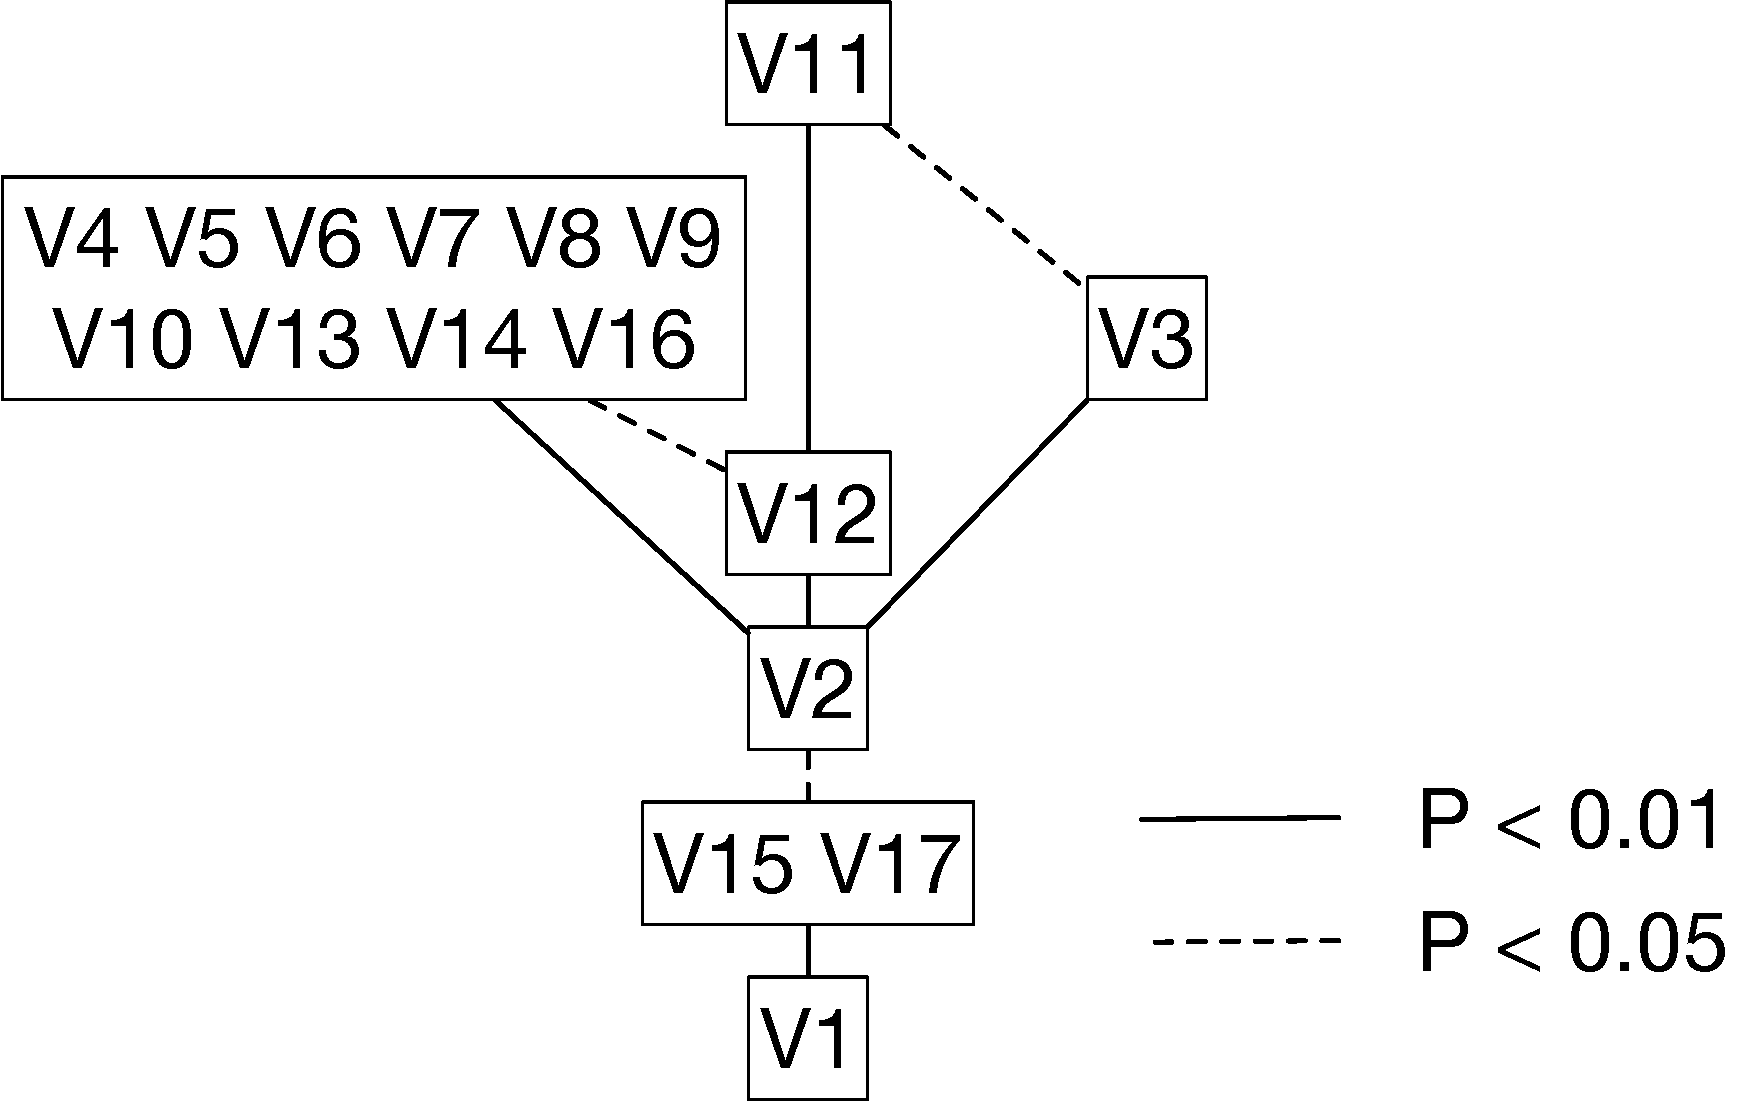
\includegraphics[width=0.8\columnwidth]{images/dominance}
\caption{Partial order dominance diagram for simulation experiments. We used Fisher's exact test.}
\label{fig:dominance}
\end{figure}

For variants V12-V14, the gradient based optimisation ran for 50 iterations, using a learning rate of 0.001 for position inputs and 0.01 for finger joints.\footnote{We used different learning rates since the parameters are in different units: position in meters and finger joint angles in radians.} For variants V15-V17 the simulated annealing procedure ran for 5 iterations, with 20 random perturbations in each step. We start with a temperature of 0.2 and halve it after every iteration. If the solution does not improve after three steps, optimisation stops. Perturbations that will result in a collision with the table are rejected.

The main findings are as follows. First, of the pure generative models GM2 outperforms GM1, with top ranked grasp successes of 79.05\% and 69.53\% respectively. Second, the joint architectures all outperform both pure GM architectures, starting at 87.85\% of grasps succeeding (V3 based on proposals from GM1 and evaluation by EM1 trained on TS1). Third, the increase in training set size (adding GM2 to GM1) yields a further improvement. We can best measure this by considering the residual number of top grasps that fail as a percentage of the baseline (GM1). On this measure adding the additional data (variants V6-V9) improves performance (over variants V3-V5) by an average of 3\%. 

The results above use GM1 as the generative model. We can measure the benefit of substituting this by GM2. This yields a further reduction in residual failures over GM1 under the same conditions (training with DS1-Tr and DS2-Tr) of 3.5\%.

\begin{figure}[t]
\centering
\subfloat[GM1 Ranking Comparison]{%
  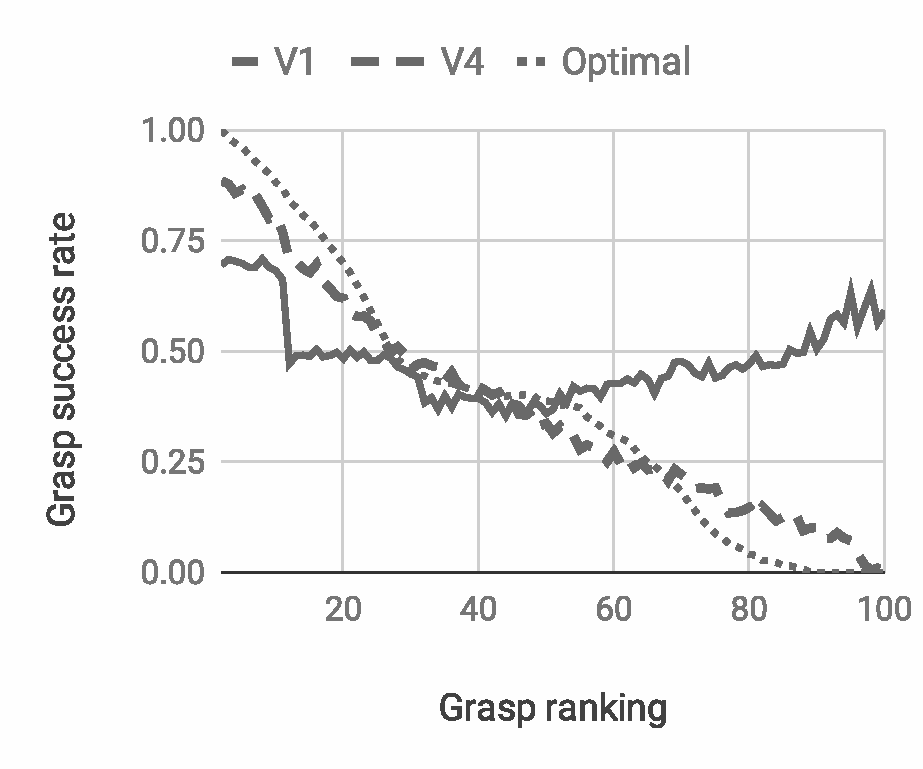
\includegraphics[width=0.45\columnwidth]{images/svr_gm1.pdf}
}

\subfloat[GM2 Ranking Comparison]{%
  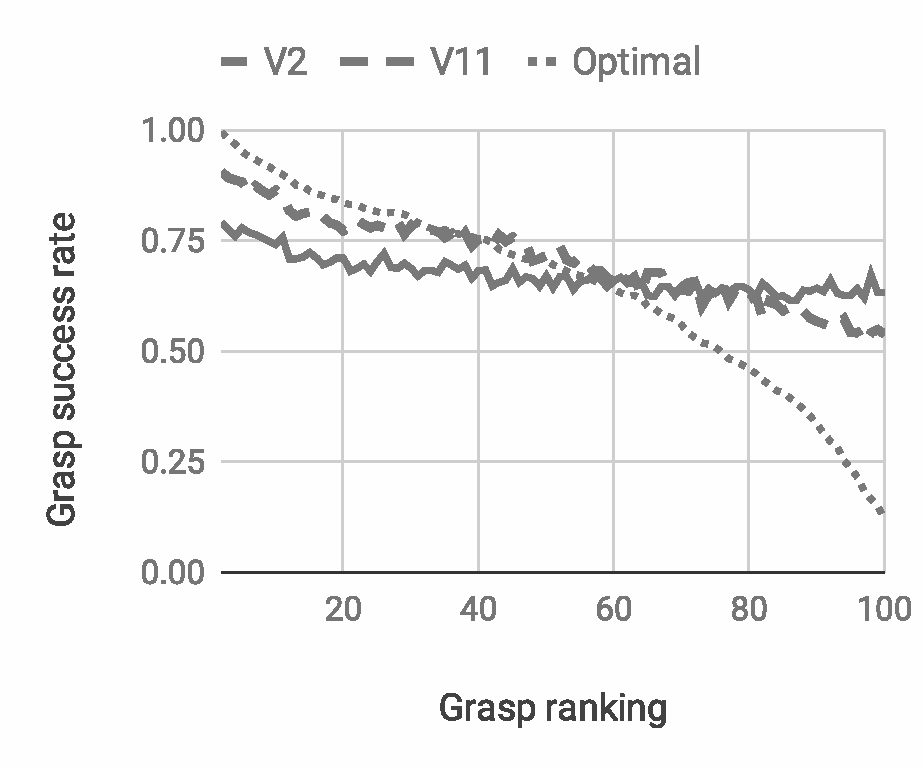
\includegraphics[width=0.45\columnwidth]{images/svr_gm2.pdf}
}
  \caption{Grasp success probability (in simulation) vs. grasp ranking. (a) GM1 vs. V4 vs. optimal ranking (empirical limit). (b) GM2 vs. V11 vs. optimal.}
  \label{fig:successvsranking}
\end{figure}


For both the gradient and simulated-annealing based optimisations, while the predicted probability of success according to the EM rises, the actual success rate in simulation declines for all variants V12-V17. We observed that wrist position changes have a greater negative impact than finger joint. The results suggest that optimising dexterous grasps by the EM is non-trivial. It should be noted that the performance of the gradient ascent was much better than the simulated annealing.

It is instructive to understand the effect of re-ranking with the EM by referring to Figure~\ref{fig:successvsranking}. This shows the average grasp success probability (across the test set) in simulation against the grasp rank. We observed that the evaluative models are much more effective than the generative models at correctly ranking the grasps. The optimal ranking is also shown. It can be seen that the GEA architectures remove more than half the residual grasp failures by re-ranking so that a good grasp is the first ranked grasp.

In summary, simulation results provide evidence that: (i) pure GM2 outperforms GM1; (ii) adding training data (DS2-Tr to DS1-Tr) improves results; (iii) using GM2 as the generative model in the generative-evaluative architecture improves results; and (iv) that post-rank tuning of the grasp using the EM output as the objective function doesn't improve results.

%Recall that the generative-evaluative architecture (GEA) comprises both the generative model (GM) and the evaluative model (EM). 
%We can evaluate aspects of these separately. After training, the EM was used to predict grasp outcomes in the test set. This comprised 1,241 scenes with 76,213 grasps. Of these, 40,243 succeeded and 35,970 failed. Our analysis is given in Table~\ref{fig:predictions}. The sensitivity is 0.84 and the specificity 0.71. The F1-score is 0.802.
%\begin{table}[b]
%\centering
%\caption{Confusion matrix for prediction on simulated data.}
%\label{fig:predictions}
%\begin{tabular}{|c|c|c|c|c|c|}
%\hline
% & & \multicolumn{4}{c|}{Prediction} \\ \cline{3-6}
%      & & \multicolumn{2}{c|}{\#} & \multicolumn{2}{c|}{\%} \\ \cline{3-6}
%  &  & Succ         & Fail         & Succ         & Fail         \\ \hline
%\multirow{ 2}{*}{Ground Truth} \newline & Succ & 33890      & 6353       & 84\%     & 16\%       \\ \cline{2-6}
% &Fail & 10339      &  25631    & 29\%     &  71\%   \\ \hline
%\end{tabular}
%\end{table}
% In this context, precision is the fraction of correctly labeled grasps among those predicted to be of a certain class (success or failure). Recall stands for the fraction of relevant grasps that have been identified correctly among all grasps that belong to that class. The results show a high recall rate for successful grasps, and there are relatively more false positives than false negatives. This necessitates pairing our evaluative neural network with a generative model rather than a random grasp generator, which would likely result in very low quality grasps and consequently, more false positives. 

%To test our generative-evaluative learning architecture we compared the grasp it proposes to the grasp proposed by the generative learner alone. Since \citet{kopicki2015ijrr} showed a 77.7\% success rate with the original generative algorithm we generated a new test set that contained both more challenging objects and placed them in challenging poses. The difficulty single-view grasping with a depth camera depends greatly on the pose of the object relative to the camera. The set comprised 40 test objects (Figure~\ref{fig:real-objects}) and another six training objects. The training objects were used by the human to demonstrate ten example grasps (Figure~\ref{fig:generative-training}). The 40 test objects were used to generate 49 object-pose pairs. From the 40 objects, 35 belonged to object classes in the simulation dataset, while the remaining five do not. 


%We compared the EM and GM rankings (Figure~\ref{fig:successvsranking}). The x-axis shows the ranking. The y-axis shows the average actual success rate over all scenes (1,241 test, 7,311 training). When ranked by the EM, the grasp success probability falls nearly monotonically, as is desirable. On the other hand, the likelihood-based ranking of GM results in many good grasps being low-ranked. We also wish to know whether the grasps recommended by the EM and the GM have different grasp success rates. The success rates of the top-ranked grasps are 71.59\% (GM) and  84.2\% (EM).

%A pure generative model architecture (GM) and the generative-evaluative architecture (GEA) were evaluated using a paired trials methodology. Each was presented with the same object-pose combinations. Each architecture generated a ranked list of grasps, and the highest ranked grasp was executed. The highest-ranked grasp based on the predicted success probability of the network is performed on each scene. A grasp was deemed successful if, when lifted for five seconds, the object then remained stable in the hand for a further five seconds before being automatically released. The success rate for GM was 57.1\% and for GEA it was 77.6\%. The successes and failures for each method were recorded and are summarised in Table~\ref{tab:robot-results}. A two-tailed McNemar test, for the difference between success rates for paired comparison data, was performed and the difference between the two algorithms has a $p$-value of 0.0442, and so is statistically significant. A selection of grasps where the two methods performed differently are shown in Figure~\ref{fig:successfail}.

% OLD TABLE
%\begin{table}
%\begin{center}
%\caption{Results of the real robot paired comparison trial.}
%\begin{tabular}{|c|c|c|c|}  \hline 
%          &                & \multicolumn{2}{ c |}{ GM} \\ \hline
%          &                & \# succs & \# fails  \\  \hline
 %GEA  & \# succs &  23 &  15  \\
 %         & \# fails    &  5   &   6   \\ \hline
%\end{tabular}
%\end{center}
%\label{tab:robot-results}
%\end{table}

%Training parameters for network. Training of example grasps for learning from demonstration. Creation of real test data set. Paired comparisons methodology with vanilla LFD algorithm (pose + object + camera view).
%
%The actual grasping tests have been performed on the real robot. 